


\documentclass{beamer}
\title{Advanced Systems Lab - Design} 
\author{Lukas Elmer, Matthias Ganz} 
\date{\today} 

\usepackage{epstopdf}



%\usetheme{Antibes}
%\usecolortheme{default}


\begin{document}


\begin{frame}
\titlepage
\end{frame} 

\begin{frame}
\frametitle{Table of content}
\tableofcontents
\end{frame} 



\section{Overview}
\begin{frame}
\frametitle{System Overview}

\begin{figure}
  \begin{center}
    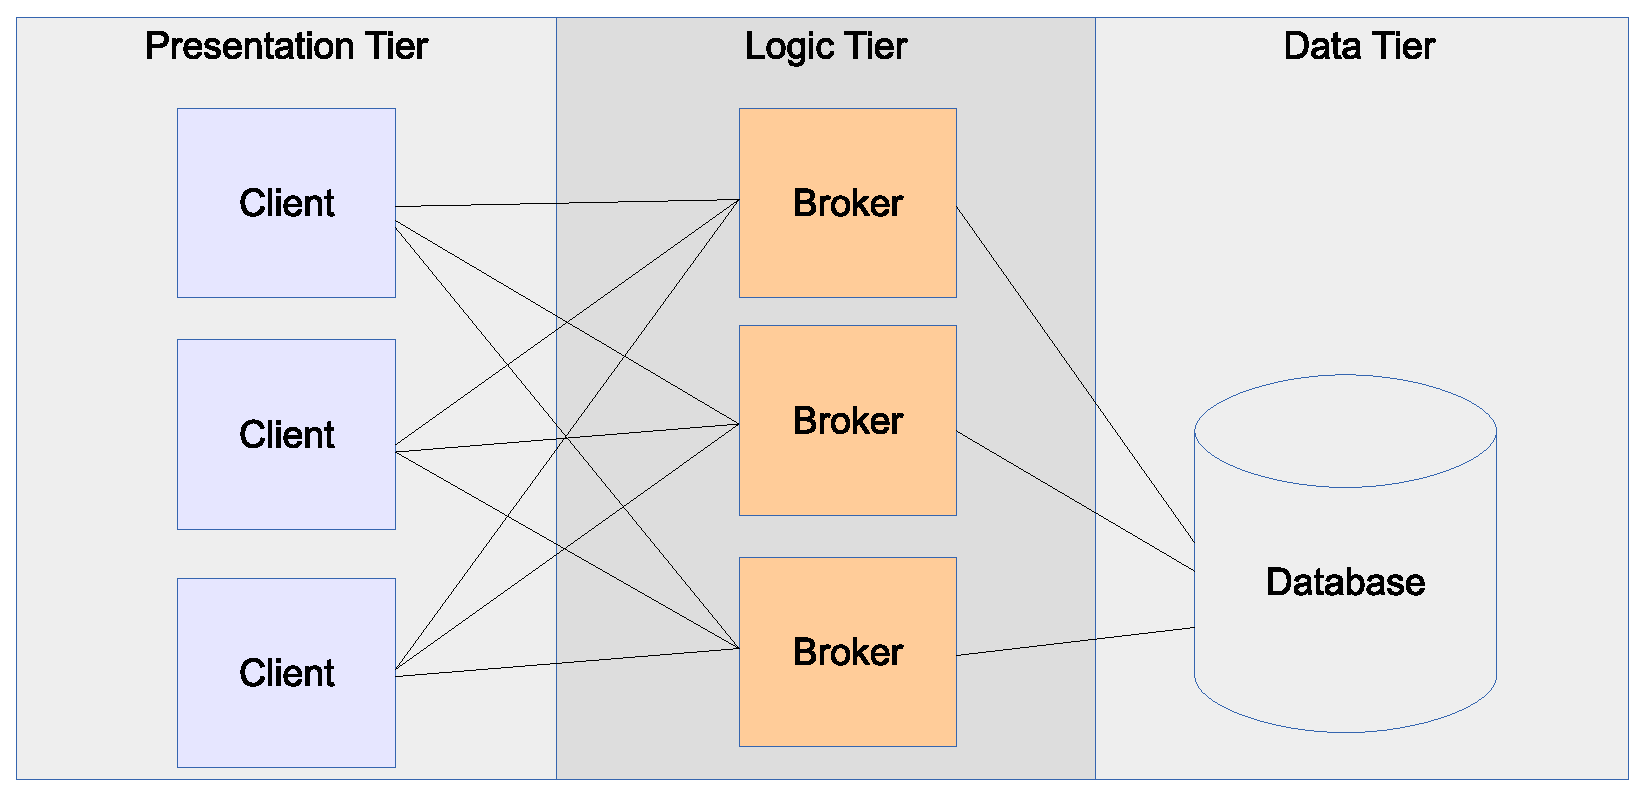
\includegraphics[scale=0.2]{../../drawings/system-overview.eps}
  \end{center}
  \caption{System Overview}
  \label{fig:system-overview}
\end{figure}

The messaging system utilizes a single database instance. On the logic tier multiple broker instances may be running. Each broker serves a certain number of clients.


\end{frame}

\section{Messaging System}

\begin{frame}
\frametitle{Broker Internals}
\begin{itemize}
\item each broker is responsible for certain queues
\item clients may ask any broker about who handles requests for a specific queue
\item a client may connect to any server number of brokers depending on which target queue it wants to send messages
\end{itemize}
\end{frame}

\begin{frame}
\frametitle{Server networking}
\begin{itemize}
\item Threading (add fancy image here)
\item Java NIO (Reactor or Leader/Followers)
\end{itemize}
http://www.kircher-schwanninger.de/michael/publications/lf.pdf
\end{frame}



\section{Database}
\begin{frame}
\frametitle{Database Schema}

\begin{figure}
  \begin{center}
    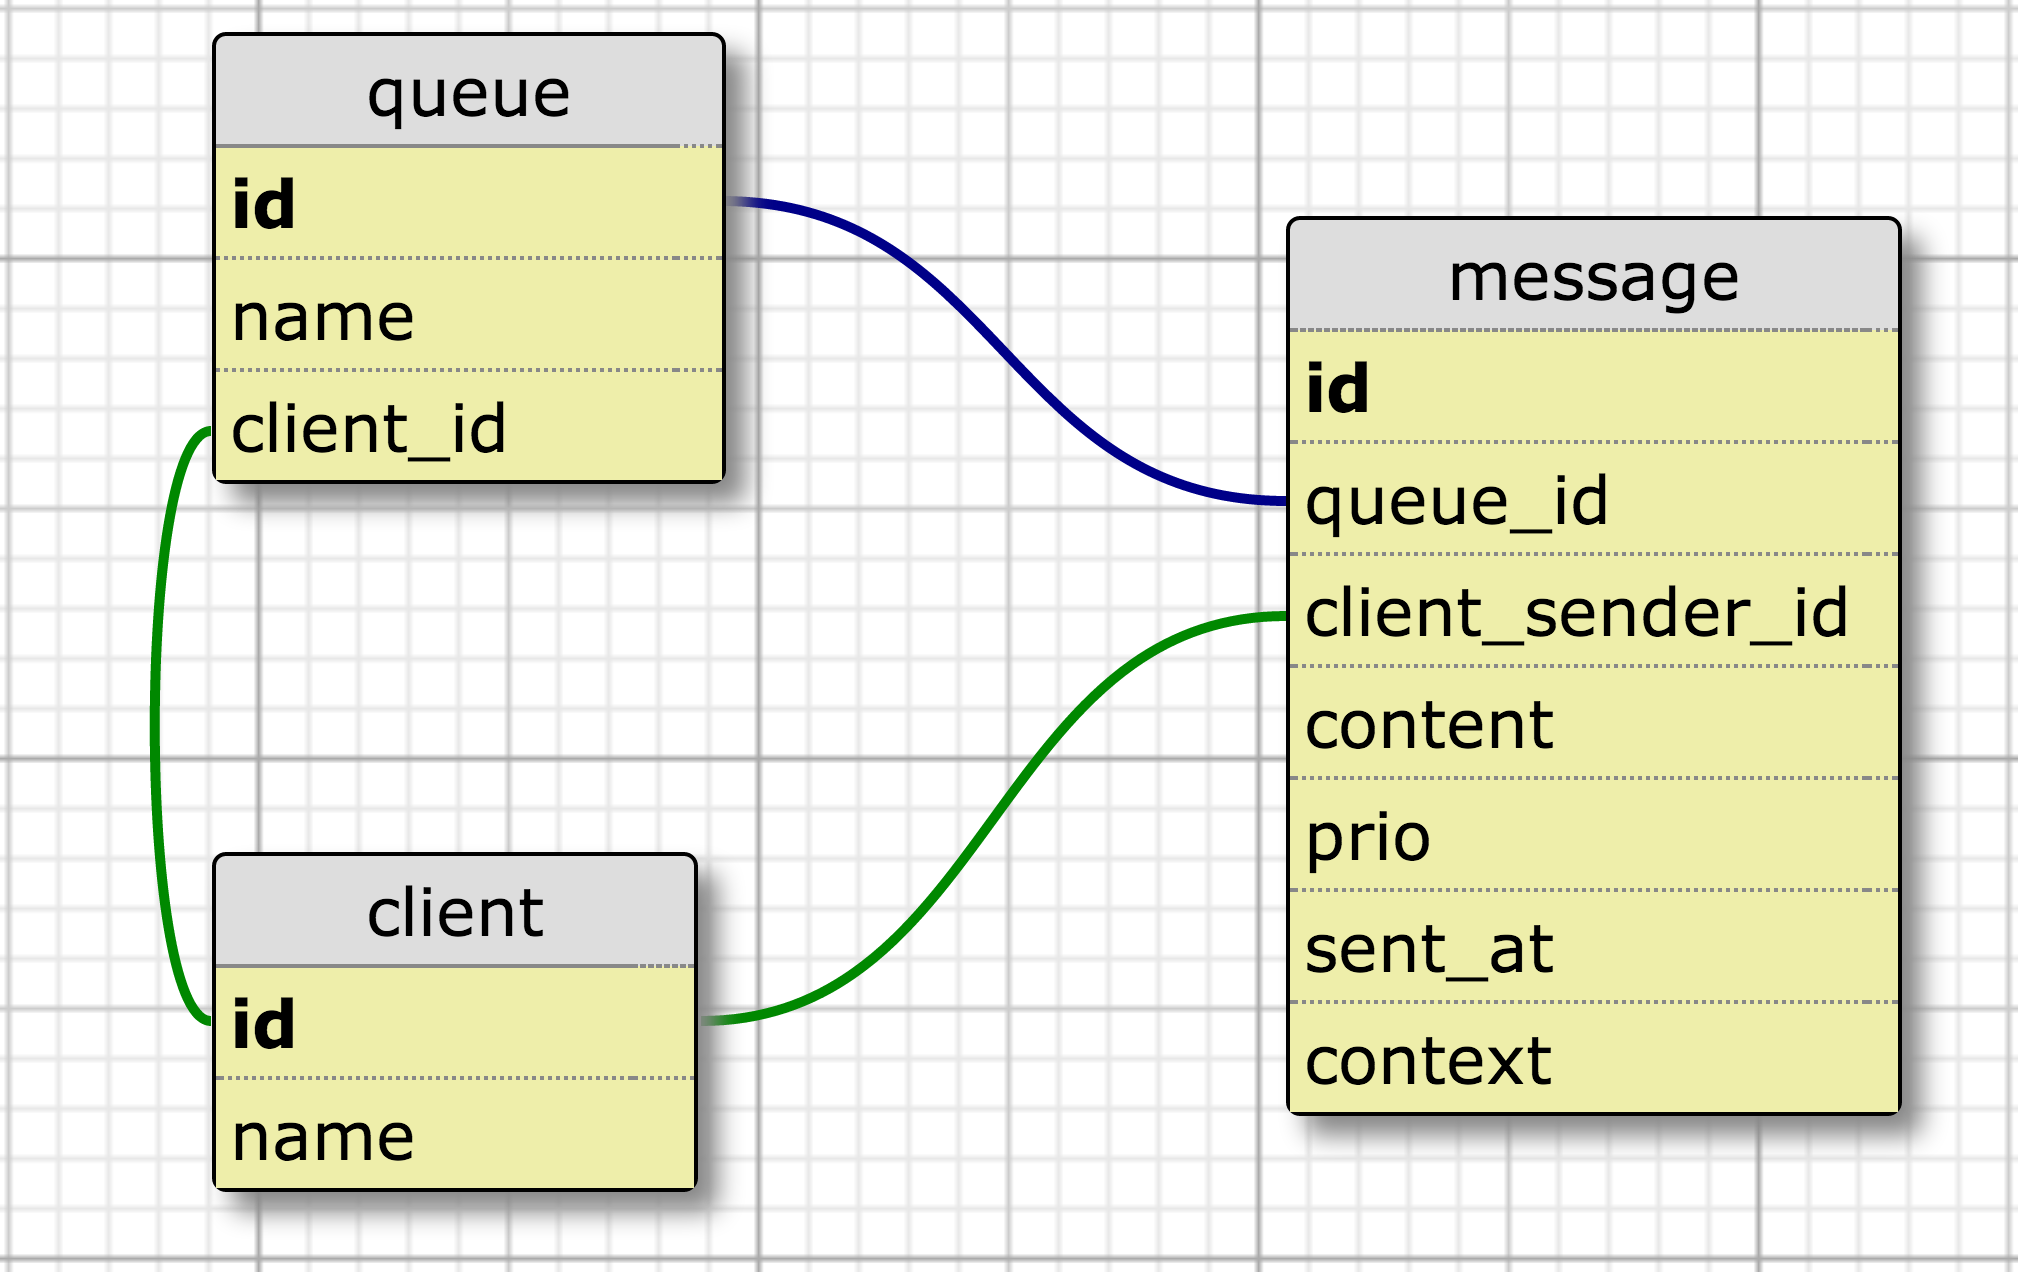
\includegraphics[scale=0.4]{../../database/db-schema.png}
  \end{center}
  \caption{Database Schema}
  \label{fig:db-schema}
\end{figure}
\end{frame}






\begin{frame}
\frametitle{Client to Broker Communication}

Describe Communication between clients and broker
\begin{itemize}
\item simplified http, only http post
\item xml over http with fixed content-length
\end{itemize}

Are we allowed to use this:
http://docs.oracle.com/javase/7/docs/jre/api/net/httpserver/
spec/com/sun/net/httpserver/HttpServer.html

HTTP in Java:
http://docs.oracle.com/javase/6/docs/jre/api/net/httpserver/
spec/com/sun/net/httpserver/HttpExchange.html

-> Problem: no keep-alive -> bad...?
\end{frame}


\begin{frame}
\frametitle{Client to Broker Communication (new)}

Describe Communication between clients and broker
\begin{itemize}
\item Serialize POJO's and send it over the network
\item Header: length of the Java object
\item Body: serialized Java object
\item Connection: keep alive, connection pool
\item Security: no authentication
\end{itemize}
\end{frame}


\section{Client}
\begin{frame}
\frametitle{Client}
Browser: good idea for development and management console.
But: cannot do many requests and measure them?
\begin{itemize}
\item May be implemented as a simple html page running in any browser
\item Management console in HTTP?
\end{itemize}
\end{frame}


\section{Client (new)}
\begin{frame}
\frametitle{Client}
\begin{itemize}
\item Different clients are implemented in Java
\begin{itemize}
\item{Only send messages}
\item{Only read messages}
\item{Only do request/response}
\end{itemize}
\item Management console in HTTP
\begin{itemize}
\item{To start/stop the current action}
\item{To collect statistics}
\end{itemize}
\end{itemize}
\end{frame}


\section{Communication Protocol}
\begin{frame}
\frametitle{Communication Protocol}
\begin{enumerate}

\item Communication Protocol used by client and server
\item Exception handling

\end{enumerate}

\end{frame}



\section{Management Interface}
\begin{frame}
\frametitle{Management Interface}
Use JMX?

\begin{itemize}

\item + little implementation effort
\item - jmx uses rmi (networking, routing issues)
\item - using a jmx gui client on the cloud might be difficult (though it's possible)

\end{itemize}
\end{frame}


\section{Measurements}
\begin{frame}
\frametitle{What experiments are performed}


\begin{enumerate}
\item what kind of experiments are performed
\item how to perform measurements
\item where to store measurement results (Format, Use DB, etc)
\end{enumerate}

\end{frame}


\end{document}

